\documentclass[11pt,twoside]{article}
\usepackage{techrep-PFG-ic}
\usepackage[english]{babel}
\usepackage[utf8]{inputenc}
\usepackage[T1]{fontenc}
\usepackage{graphicx}
\usepackage{amsmath}
\usepackage{amssymb}
\usepackage{subfigure}
\usepackage{url}
\usepackage{array}
\usepackage{multirow}
\usepackage{tabularx}
\usepackage{colortbl}
\usepackage[table,xcdraw]{xcolor}
\usepackage{textcomp}
\usepackage{verbatim}
\usepackage{setspace}
\usepackage{geometry}
\usepackage{float}
\usepackage{enumitem}
\usepackage{ dsfont }

\begin{document}

\TRNumber{20}

\TRYear{19} 
\TRMonth{06} 


\TRAuthor{A. C. Corrales \and A. M. Idalgo \and L. A. Racoci \and G. A. R. Rivera}

\TRTitle{Combinatory Study\\on Graph Network Predictions}

\TRMakeCover

%%%%%%%%%%%%%%%%%%%%%%%%%%%%%%%%%%%%%%%%%%%%%%%%%%%%%%%%%%%%%%%%%%%%%%
% O que segue é apenas uma sugestão - sinta-se à vontade para
% usar seu formato predileto, desde que as margens tenham pelo
% menos 25mm nos quatro lados, e o tamanho do fonte seja pelo menos
% 11pt. Certifique-se também de que o título e lista de autores
% estão reproduzidos na íntegra na página 1, a primeira depois da
% página de capa.
%%%%%%%%%%%%%%%%%%%%%%%%%%%%%%%%%%%%%%%%%%%%%%%%%%%%%%%%%%%%%%%%%%%%%%

%%%%%%%%%%%%%%%%%%%%%%%%%%%%%%%%%%%%%%%%%%%%%%%%%%%%%%%%%%%%%%%%%%%%%%
% Nomes de autores ABREVIADOS e titulo ABREVIADO,
% para cabeçalhos em cada página.
%
\markboth{Corrales, Idalgo, Racoci and Adin}{Combinatory Study}
\pagestyle{myheadings}


\title{Combinatory Study on Graph Network Predictions}

\author{
    Alan Corrales
    \and Allana Idalgo
    \and Lucas Racoci
    \and Adín Ramírez
    \thanks{Institute of Computation, State University of Campinas, 13081-970  Campinas}
}

\date{}

\maketitle

\begin{abstract}
To test Deepmind's Graph Nets framework against invariance properties defined by [citation] in graphs representation, we used three different problems in at least four different scenarios each: with and without permutations in the representation of entries of train and test sets.

In all those scenarios, the common behavior was that permuting test sets affected way less the results than permuting training. These results reinforce the argument that the algorithms might not be learning from the graph structure itself, but from the graph computational representation.
\end{abstract}



\section{Introduction}

\subsection{Overview}
Artificial Intelligence has gone through a renaissance with progress on computer vision, natural language processing, automation and control and decision problems ~\cite{Battaglia_2018}. Since 1986 ~\cite{Rumelhart_1986} and mainly after 2006 ~\cite{Hinton_2006}, Artificial Neural Networks has begun to stand out along with variations of Convolutional Neural Networks (CNNs) and Recurrent Neural Networks (RNNs).


\begin{figure}[!htb]
    \centering
    \subfigure[Fully connected]{
        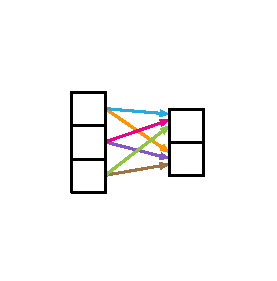
\includegraphics[height=3.0cm]{fig/content/intro/simple_neural_network/fully_connected.pdf}
    }
    \subfigure[Convolutional]{
        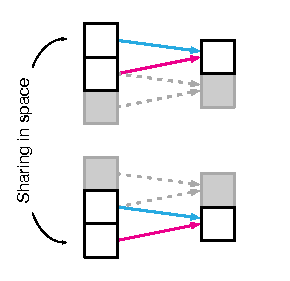
\includegraphics[height=3.0cm]{fig/content/intro/simple_neural_network/convolutional.pdf}
    }
    \subfigure[Recurrent]{
        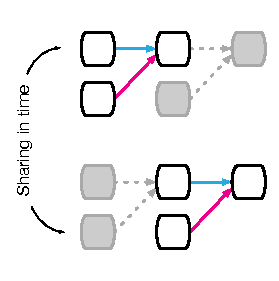
\includegraphics[height=3.0cm]{fig/content/intro/simple_neural_network/recurrent.pdf}
    }
    \caption{Simplified representation of some neural networks models ~\cite{Battaglia_2018}}

    \label{fig:simple_neural_network}
\end{figure}

Recently, between 2017 and 2018, papers ~\cite{Battaglia_2018, Gilmer_2017, Wang_2018} describing generalized graph prediction algorithms were published. These would provide a framework for predicting, with some acceptable error, output graphs given input graphs. Applications of these solutions varies from modelling molecular structures in Chemistry to Corpuscular Mechanics, and Community Studies.

In 2019, January 2nd a broad review ~\cite{Zhou_2019} of the main graph networks algorithms was carried out confirming that the Graph Nets’ approach ~\cite{Battaglia_2018} generalizes the Message Passing Neural Network ~\cite{Gilmer_2017} and Non Local Neural Network ~\cite{Wang_2018}, which by themselves were generalizing a lot of other methods. Some of those methods will be further detailed in the next section. This review presents the three cited algorithms. 


\subsection{Invariant Networks}

Given a graph $G = (V, A)$ consisting of $n$ nodes $V$ and values $A$ attached to its edges (in this case, an edge is an ordered subset of the nodes V).

When constructing a functional relation $f(A^l) \approx T^l$, where $f$ is a neural network and $T^l$ are the corresponding targets, if $f$ is order invariant, then it should produce the same output regardless of the node numbering used to encode $A$.

For example: Given an arbitrary adjacency matrix $A = A \in \mathds{R}^{n \times n}$, representing the graph. For an arbitrary permutation matrix $P$, the function f is order invariant if it satisfies $f(P^T A P) = f(A)$.

Since the neighborhood aggregation approach is as powerful as the Weisfeiler-Lehman graph isomorphism test ~\cite{Xu_2018}, we conjectured that the the Graph Nets’ approach would not be order invariant which would reflect in limitations on the algorithms’ performance when dealing with copies of a graph but permuted in representation. 
\section{Graph Networks}

\subsection{Message Passing Neural Networks}

Gilmer et al. describes Message Passing Neural Networks (MPNN) as a framework that generalizes at least eight models found in the literature ~\cite{Gilmer_2017}. The MPNN method describes a messaging and a readout phase on forward propagation, as shown in Fig.\ref{fig:mpnn}.
	
The hidden nodes, $h_v^t$, are updated based on messages $m_v^{t+1}$, for a number of timesteps.

\begin{equation}
    \label{eqn:message}
    m^{t+1} = \sum_{w \in N(v)} M ^ {T} (h^t_v, h^t_w, e_{vw})
\end{equation}

\begin{equation}
    h^{t+1} = U_t(h^t_v, m^t_v)
\end{equation}

\begin{equation}
    \hat{y} = R (\{h^t_v | v \in G\})
\end{equation}

According to Battaglia et al.~\cite{Battaglia_2018}, the MPNN framework can be adapted to GN formalism. The exact translation is described as:

\begin{itemize}

    \item The message function, $M^{t}$, corresponds to the GN’s $\phi ^ e$, but does not take $u$ as input,
    
    \item Element wise summation is used for the GN’s $\rho ^ {e \rightarrow v}$,
    
    \item The update function, $U_t$, is translated to the GN’s $\phi ^ v$
    
    \item The readout function, $R$, plays the role of the GN’s $\phi ^ u$, but does not take $u$ or $E'$ as input, and thus an analog to the GN’s $\rho ^ {e \rightarrow u}$ is not required;
    
    \item $d_{\text{master}}$ serves a roughly similar purpose to the GN’s $u$, but is defined as an extra node connected to all others, and thus does not influence the edge and global updates directly. It can then be represented in the GN’s $V$.

\end{itemize}

\begin{figure}[H]
    \centering
    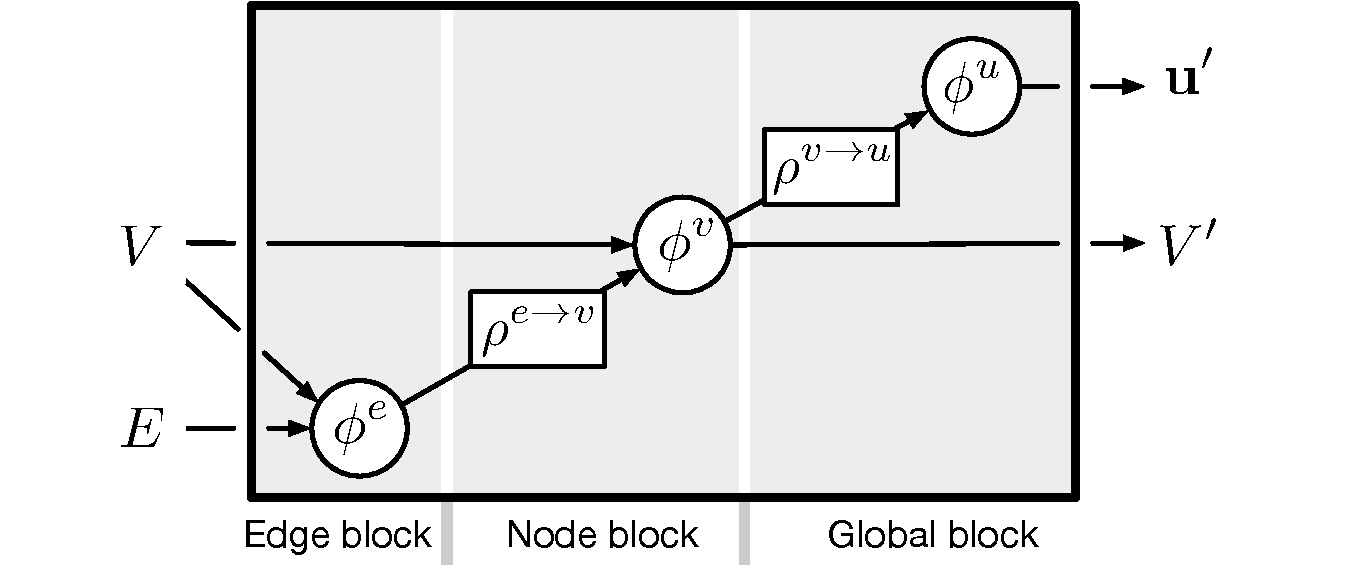
\includegraphics[width=.7\textwidth]{fig/content/graph_nets/blocks/mpnn.pdf}
    \caption{The forward pass phases of the Message Passing block elicited above ~\cite{Battaglia_2018}.}
    \label{fig:mpnn}
\end{figure}



\subsection{Non Local Neural Networks}

Both recurrent and convolutional operations are building blocks that process one local neighborhood at a time. On the other hand, fully connected layers have those relations encoded in the learned weights, therefore the relationship between the points is not a direct function of the input layer. 

Non Local Neural Networks (NLNN) ~\cite{Wang_2018} present mid-term building blocks for capturing long-range dependencies. In it, the forward pass is computed by repeatedly applying a weighted sum of a function of the previous step, but in this case, part of the weight is a similarity measure ($f$) between the node being calculated and the node being summed over.

\begin{equation}
    h^{t+1}_v = 
    \cfrac{1}{C(h^t)} 
    \cdot \sum_{\forall u \in V} {
        f(h^t_v,h^t_u) \cdot g(h^t_u)
    }
\end{equation}
The NLNN framework can be adapted to GN formalism ~\cite{Battaglia_2018} as follows:

\begin{itemize}

    \item Both the similarity function $f$ and the update function $g$ can be interpreted as components of the $\phi^e\left(\mathbf{e}_k, \mathbf{v}_{r_k}, \mathbf{v}_{s_k}\right) = \mathbf{e}'_k$  where $\mathbf{e}'_k = \left(\mathbf{v'}_{r_k}, \mathbf{v'}_{s_k} \right) $, $\mathbf{v'}_{r_k} = f\left(\mathbf{v}_{r_k}, \mathbf{v}_{s_k} \right)$ and $\mathbf{v'}_{s_k} =  g\left(\mathbf{v}_{s_k}\right)$, in this case $\mathbf{u}$, the universal features are not used in the edge update function $\phi^e$. 
    
    \item Weighed average is used for the GN’s 
    \begin{equation}
        \rho^{e \rightarrow v}
        \left( 
            E'_i 
        \right) 
        = \cfrac{1}{
            \sum_{
                \{ k : r_k = i \}
            } {
                \mathbf{v'}_{r_k}
            }
        }
        \cdot
        \sum_{\{k:\, r_k=i\}} \mathbf{v'}_{r_k} \cdot \mathbf{v'}_{s_k}
    \end{equation}

\end{itemize}

The NLNN block is perhaps better illustrated by Fig. \ref{fig:nlnn}

\begin{figure}[H]
    \centering
    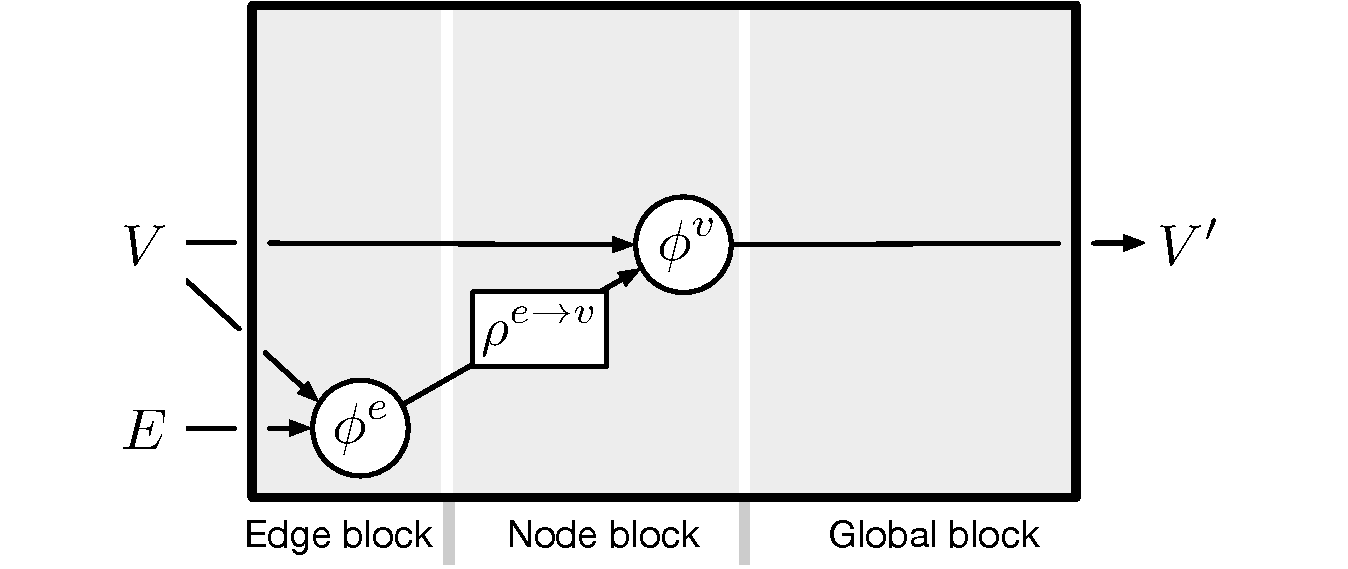
\includegraphics[width=.7\textwidth]{fig/content/graph_nets/blocks/nlnn.pdf}
    \caption{The forward pass phases of the Non Local Neural Network block ~\cite{Battaglia_2018}.}
    \label{fig:nlnn}
\end{figure}



\subsection{Graph Independent}

The Graph Independent module applies models to the graph elements independently, i.e., the models are applied to each element of the graph (nodes, edges and globals) in parallel regardless of other elements, as shown in Fig.\ref{fig:independent}.

\begin{figure}[H]
    \centering
    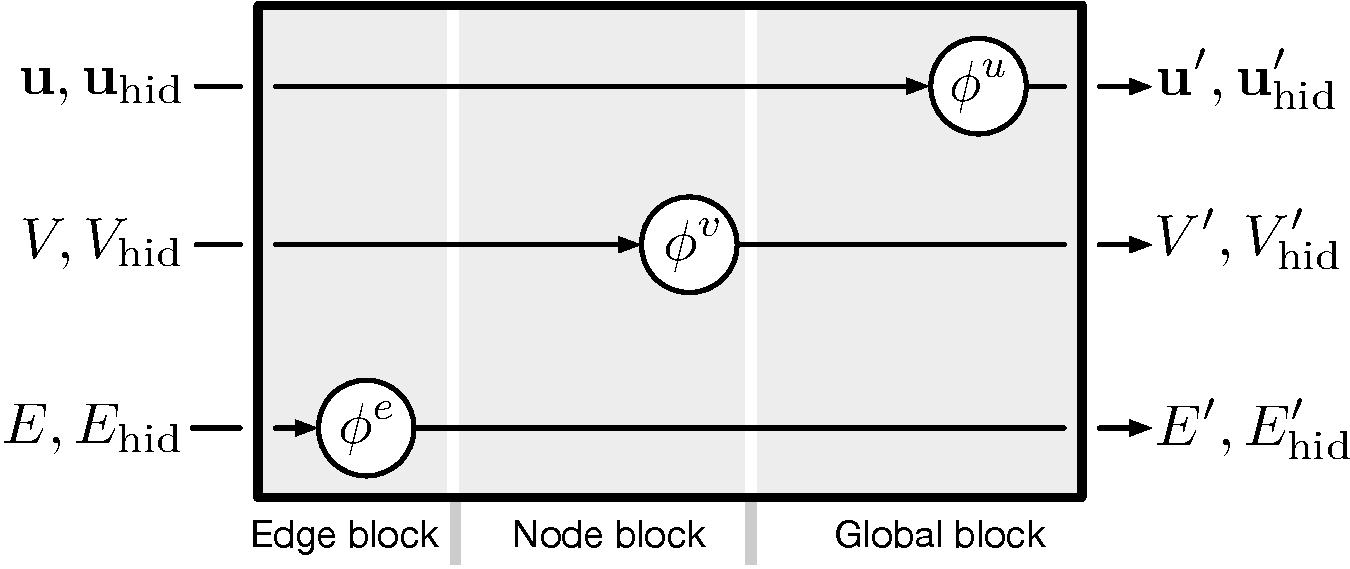
\includegraphics[width=.7\textwidth]{fig/content/graph_nets/blocks/independent.pdf}
    \caption{The forward pass phases of the Graph Independent block ~\cite{Battaglia_2018}.}
    \label{fig:independent}
\end{figure}

\subsection{Graph Nets}

The Graph Networks (GN) framework generalizes and extends various graph neural network approaches, such as MPNN and NLNN. A Graph Net is composed of blocks which operate a sequence of steps according to its configuration. One possible configuration, a full GN block Fig.\ref{fig:graph_nets_flexibility}(a), predicts node, edge, and global features based on its incoming nodes, edges, and global features.

Graph Nets framework encompasses flexible representations, configurable in-block structure and composable multi-block architectures ~\cite{Battaglia_2018}. This is shown in the block arrangements in Fig. \ref{fig:graph_nets_flexibility}. In each block, $\phi$ functions may be applied to incoming attributes and $\rho$ functions to aggregate them, generating new, updated output values (shown as either $u'$, $V'$ or $E'$).

\begin{figure}[H]
    \centering
    \subfigure[Full block]{
        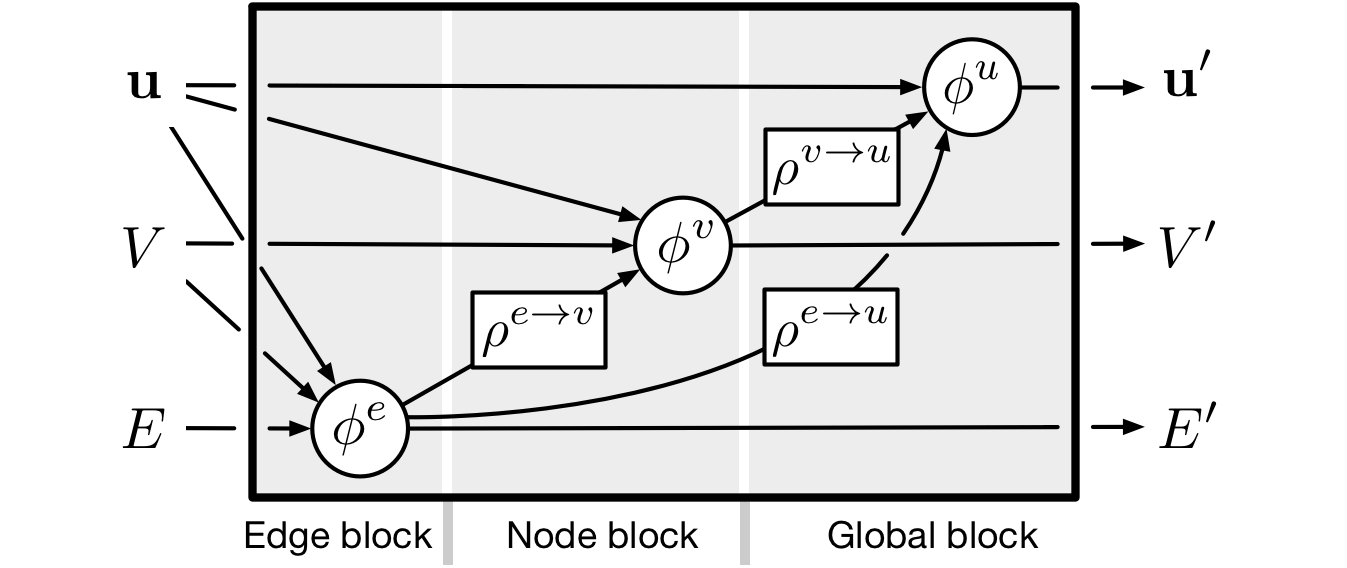
\includegraphics[width=.45\textwidth]{fig/content/graph_nets/blocks/full.png}
    }
    \subfigure[Independent block]{
        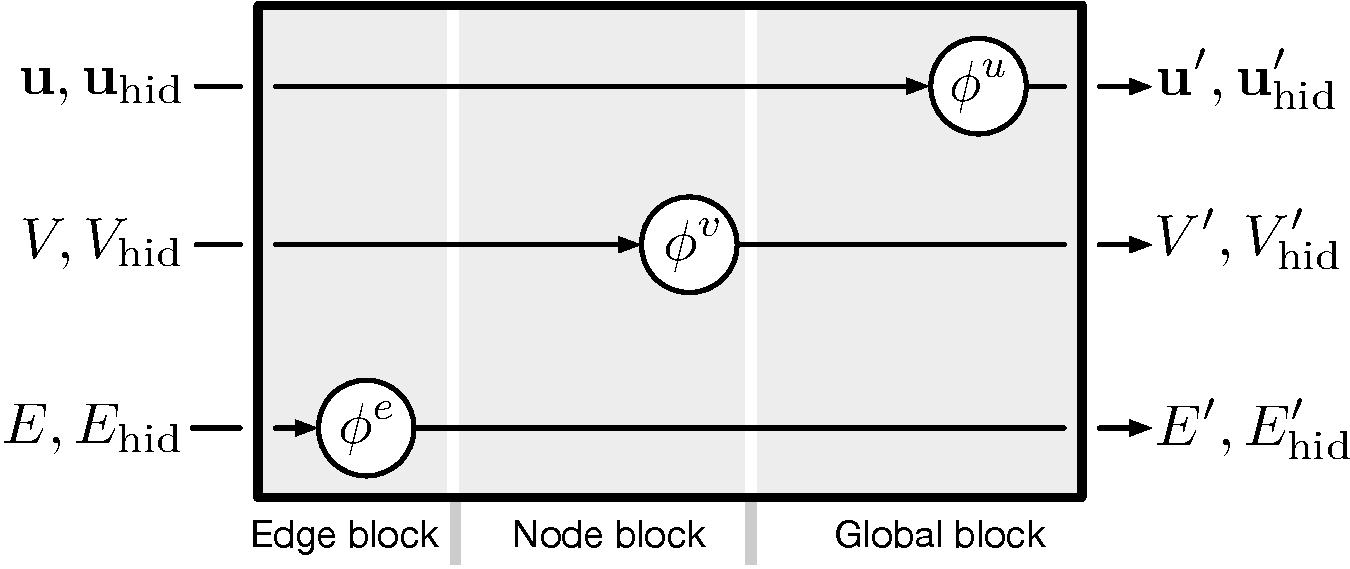
\includegraphics[width=.45\textwidth]{fig/content/graph_nets/blocks/independent.pdf}
    }
    \subfigure[Message-passing block]{
        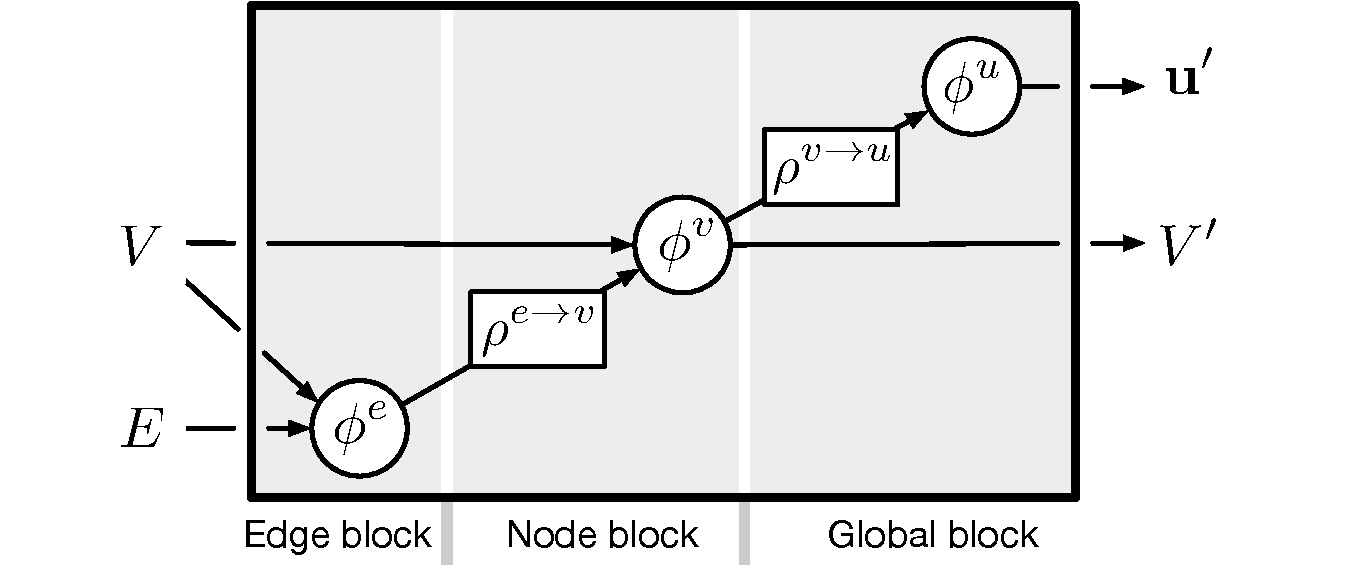
\includegraphics[width=.45\textwidth]{fig/content/graph_nets/blocks/mpnn.pdf}
    }
    \subfigure[Non Local block]{
        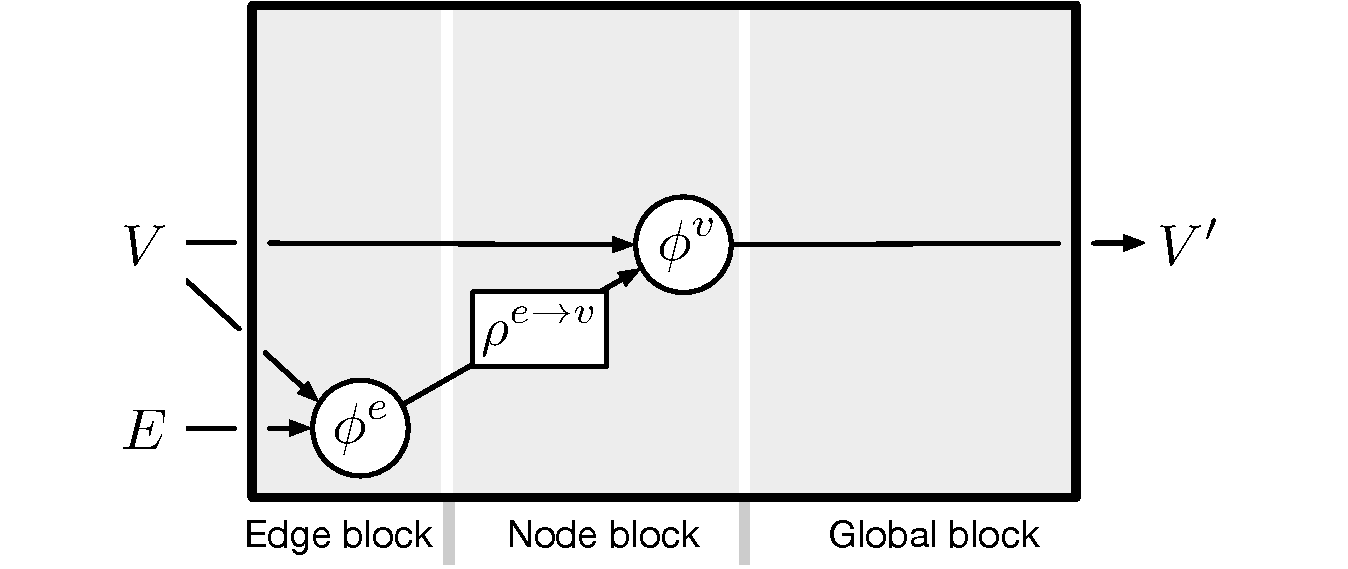
\includegraphics[width=.45\textwidth]{fig/content/graph_nets/blocks/nlnn.pdf}
    }
    
    \caption{Graph Nets internal block configurations ~\cite{Battaglia_2018}}
    
    \label{fig:graph_nets_flexibility}
\end{figure}




\section{Analyzed Problems}


\subsection{State Prediction of a Spring-mass System}

This problem explores a computational simulation derived from an actual physics experiment. Given a set of masses connected by springs, with two of them fixed, the problem is to predict the next state of the system (position and velocity of the masses) after some noise is applied.

The system always starts from rest position, with all masses in the same vertical position and zero velocity in the two dimensions.

A computational simulation of this system was carried out in Battaglia et al. (2016)'s "interaction networks" ~\cite{Bataglia_2016}. In the simulation, a random dataset is generated by initializing nodes with fixed spacing among them, and then applying noise on every timestep.

Computational representation translates masses into nodes and springs into edges. The vertex feature array is composed by $(x, y, v_x, v_y, fixed)$, where $x$, $y$ denote position, $v_x$, $v_y$ denote velocity and $fixed$ denotes whether a mass is fixed.

The edges’ feature array is composed by the springs’ rest distance and their constants, and the global feature array is composed by the gravitational acceleration. The model generates a trajectory by applying noise at each iteration of the simulation, as shown in Fig.\ref{fig:physics_trajectory}.

\begin{figure}[H]
    \centering
    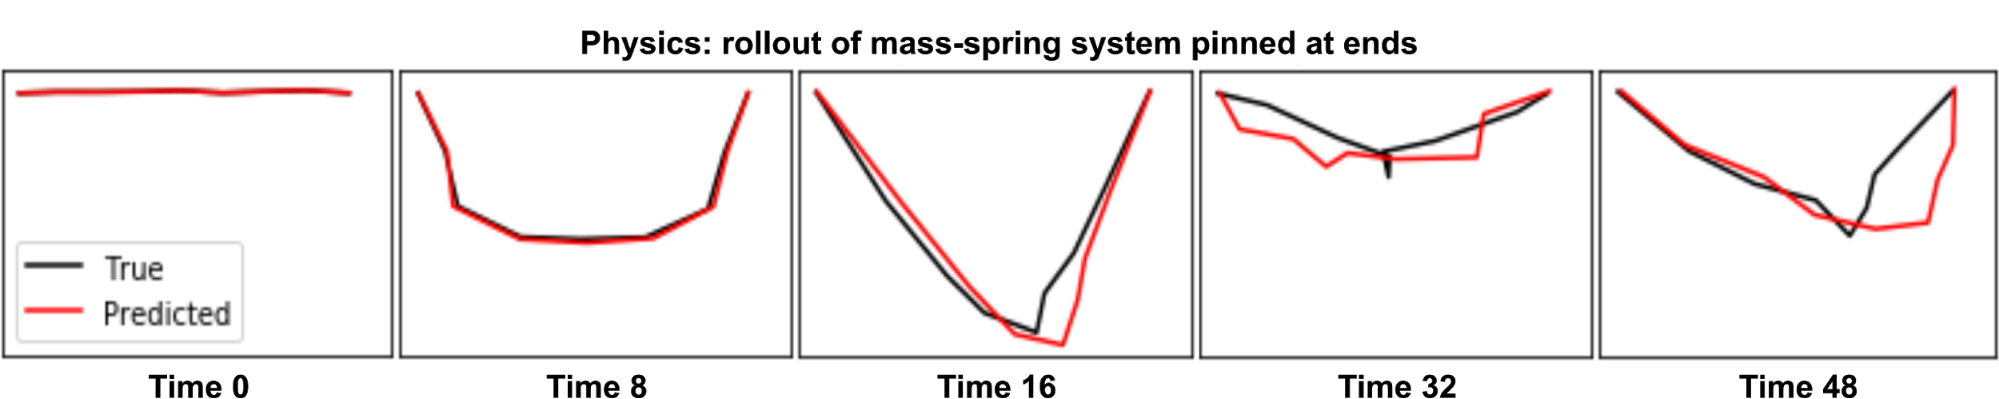
\includegraphics[width=.7\textwidth]{fig/content/analysed_problems/physics/tragectory.png}
    \caption{Predicted and true values from states along a spring-mass trajectory ~\cite{Battaglia_2018}.}
    \label{fig:physics_trajectory}
\end{figure}


\subsection{Shortest Paths}

The experiment creates random graphs, and trains a graph network to label the nodes and edges on the shortest path between any two nodes. Over a sequence of message-passing steps, the model refines its prediction of the shortest path, as shown in Fig.\ref{fig:shortest_path}.

\begin{figure}[H]
    \centering
    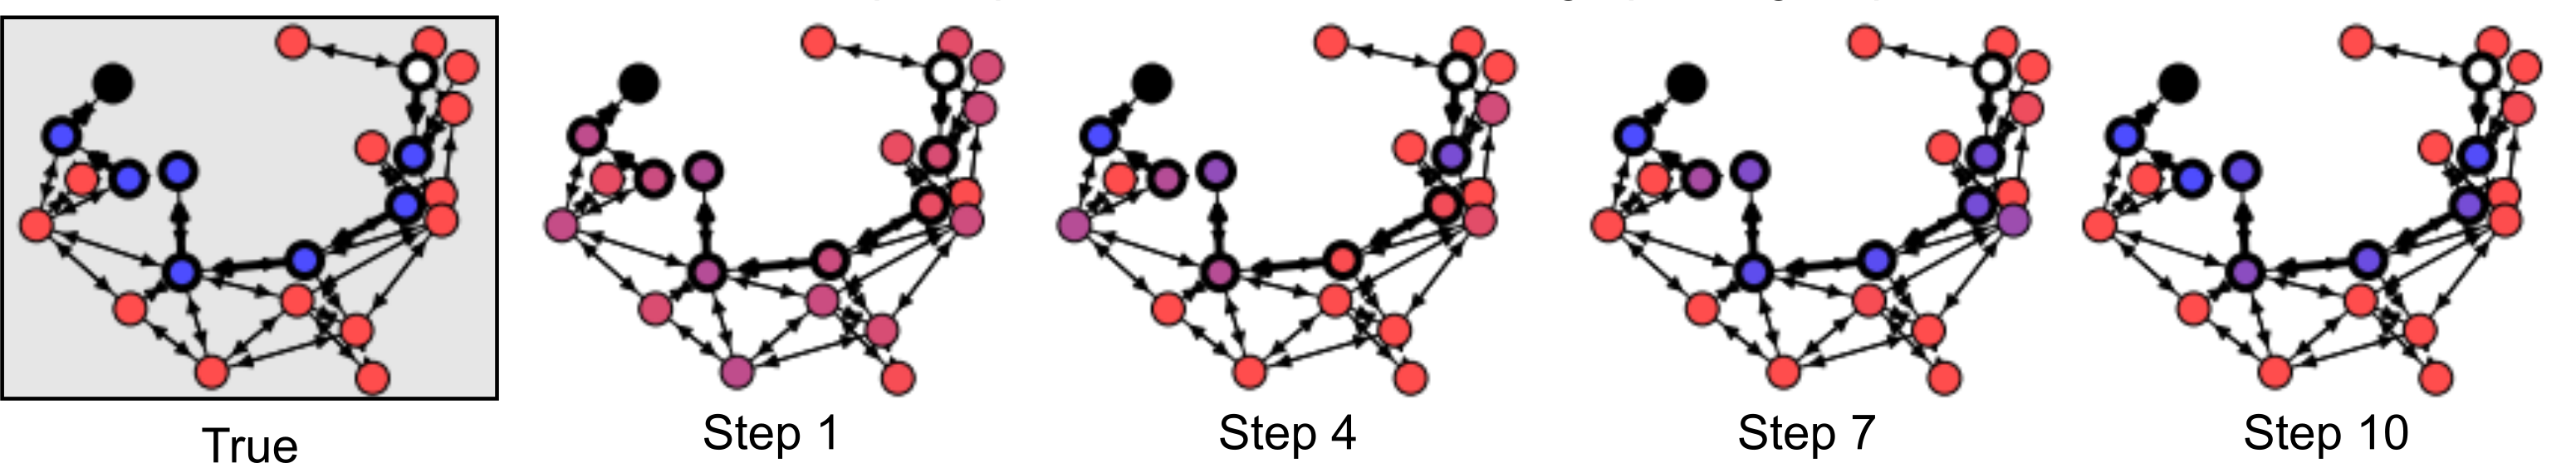
\includegraphics[width=\textwidth]{fig/content/analysed_problems/shortest_paths/steps.png}
    \caption{Prediction at each message-passing step for shortest path problem ~\cite{Battaglia_2018}.}
    \label{fig:shortest_path}
\end{figure}


\subsection{Regions Separation}

The problem is the classification of pixels of an input image, given its similarities with its neighbors. At first glance, this problem might not seem related with a graph to graph problem, but we can make a reduction of this problem to one of finding a set of independent connected components that represent each of the different classes of pixels. 

The input is transformed into a graph with one vertex for each pixel and one edge for each pair of neighbor pixels. The output can be transformed simply by partitioning the graph with a Depth First Search (DFS) or using the vertex class feature that the reduced problem must also provide.

The problem that we explored is the reduced one. The input of the reduced problem is the graph described above, with features indicating color and position in each vertex. The output of the reduced problem is the graph with vertices of different regions in different connected components and with features indicating in what region the vertex is. 

Since the set of edges in the solution is always a subset of the edges in the input, we used an edge feature to indicate if the corresponding edge is part of the solution.

A better visualisation of those problems can be seen in Fig. \ref{fig:regions_separation_dataset_visualization} with the input and output images of the original problem overlaid by the input and output graphs of the reduced problem.

\begin{figure}[H]
    \centering
    
    \subfigure[Input image and associated graph]{
        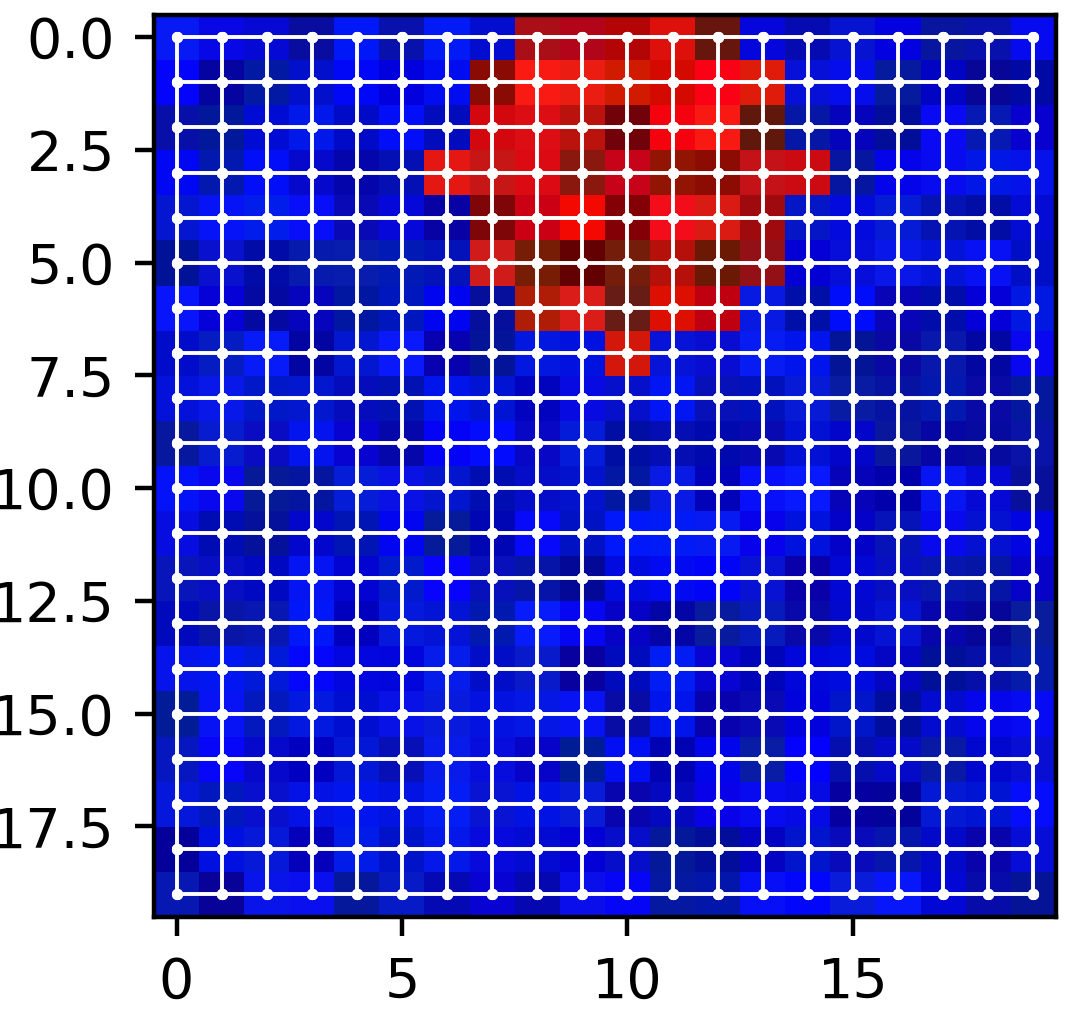
\includegraphics[width=.45\linewidth]{fig/content/analysed_problems/shapes/input.png}
    }
    \subfigure[Expected image and associated graph]{
        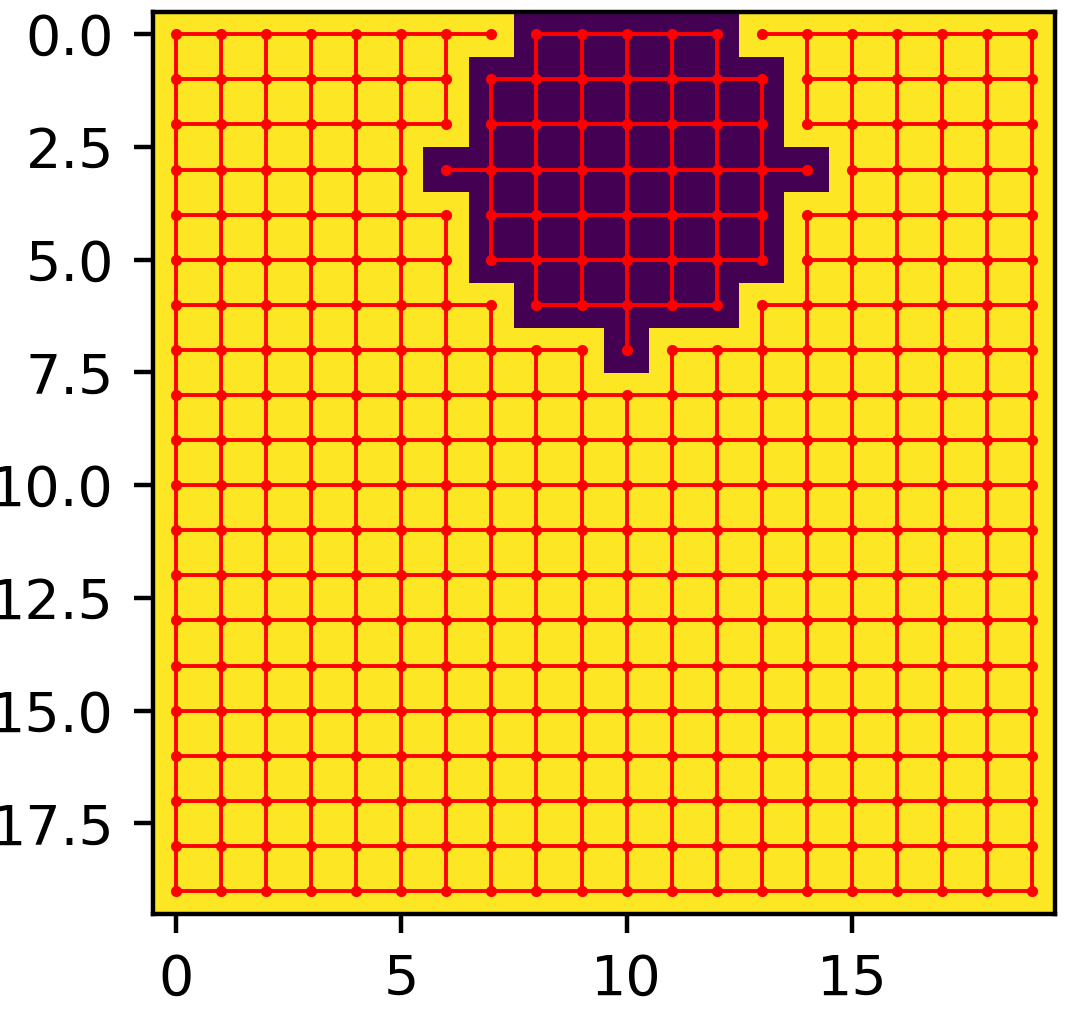
\includegraphics[width=.45\linewidth]{fig/content/analysed_problems/shapes/expected.png}
    }
    
    \caption{Visualization of an entry of the dataset used for the Region Separation problem}
    
    \label{fig:regions_separation_dataset_visualization}
\end{figure}


\section{Methodology}

The experiments used a full encode-process-decode model (Fig.\ref{fig:model}). That is, the model included three components:

\begin{itemize}

    \item Encoder: the Graph Independent module, which independently encodes the nodes, edges and global attributes
    
    \item Core: the Graph Network (GN) module, which performs N rounds of message-passing processing steps. The input is the concatenation of the Encoder’s output and the Core’s previous output.
    
    \item Decoder: the Graph Independent module, which independently decodes nodes, edges and global attributes on each message-passing step.

\end{itemize}

\begin{figure}[H]
    \centering
    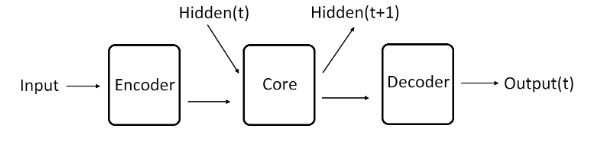
\includegraphics[width=.7\textwidth]{fig/content/model/model.jpg}
    \caption{The model}
    \label{fig:model}
\end{figure}

We used supervised learning to train the model. 

The training loss is computed on the output of each processing step. This encourages the model to solve the problem in the minimum number of steps, and helps to interpret the output of intermediate steps.

The testing loss is computed only on the final processing step and evaluates how well the model generalizes to graphs that are larger than those it was trained with.

The experiments consisted of:

\begin{enumerate}[label=(\Alph*)]

    \item Training on non-permuted data and testing on both non-permuted  and permuted data.
    
    \item Training on permuted data and testing on both non-permuted and permuted data.

\end{enumerate}

In all the experiments we used a learning rate of $10^{-3}$ running for 5 different seeds with different numbers of iterations.

\subsection{Physics Experiments}

Training data examples have 5 to 8 masses, while testing data have 4 to 9 masses. The default parameters were used, with $10^5$ training iterations, training and testing batch sizes of 256 and 100, respectively.

Permutations were applied to the senders, receivers and node features' array.

Sum of squared error was used to calculate loss at each evaluation. Accuracy was not calculated.

\subsection{Shortest Paths Experiments}

This experiment used geographic threshold graphs with added edges (using a minimum spanning tree algorithm) to guarantee that all nodes are connected. Attributes that indicates the shortest path from A to B were added to the graph. From this graph, called raw graph, we get the source and target graphs which are fed to the model described above.

The training graphs have a range of number of nodes from 8 to 17, and for the testing graphs we have a range of 16 to 33. The batch sizes are 5, for training, and 100, for testing.

The loss were computed using Softmax Cross Entropy from TensorFlow. The optimizer we used were the Adam Optimizer, also from TensorFlow. These were the default parameters used by the model from Graph Nets.

\subsection{Regions Separation Experiments}

To produce the input graph, we first generated an image consisting of two shapes in different colors with a random noise applied to the whole image.

The input graph nodes were created for each pixel of the image and from each pixel was extracted horizontal and vertical position along with red, green and blue channels as node features.

The input graph edges were created by connecting vertices with adjacent pixels, using 4-connectivity. The target graph is similar. The edge features indicates if the respective edge is part of the solution.

An edge is considered to be part of the solution if the two corresponding pixels are from the same region of the image, if they have the same color before the applied noise.

The training graphs have the number of nodes taken from a uniform distribution in the range from 8 to 17, and for the testing graphs we have a range of 16 to 33. The batch sizes are 5, for training, and 100, for testing. We used an epoch with 25 iterations, testing every 3 iterations in a simple and a permuted graph. In total the algorithm ran through 125 iterations, so 5 epochs.

The loss were computed using Softmax Cross Entropy from TensorFlow. The optimizer we used were the Adam Optimizer, also from TensorFlow.

\section{Results and Discussion}

For the loss plots, we used:

    \begin{itemize}
        \item Ltr: training loss
        \item Lge: testing/generalization loss
        \item Lpe: permuted testing/generalization loss
        \item Lge4: testing/generalization loss with 4 masses
        \item Lpe4: permuted testing/generalization loss with 4 masses
        \item Lge9: testing/generalization loss with 9 masses
        \item Lpe9: permuted testing/generalization loss with 9 masses
    \end{itemize}
    
And for the accuracy plots, we used:

    \begin{itemize}
        \item Str: training graphs solved correctly
        \item Sge: testing/generalization graphs solved correctly
        \item Spe: permuted testing/generalization graphs solved correctly
        \item Ctr: training graph elements correctly labeled
        \item Cge: testing/generalization graph elements correctly labeled
        \item Cpe: permuted testing/generalization graph elements correctly labeled
    \end{itemize}

\subsection{Experiments A - Physics}

\subsubsection {Permutation of the testing set}

This experiment was carried out to compare the network’s performance on testing with a dataset and its permuted version. The results of this setup are shown in Fig.\ref{fig:physics_base_results} with a logarithmic scale indicating the training and testing losses (both baseline and permuted).

The loss plot (Fig.\ref{fig:physics_base_results}) exhibits higher loss for Lpe4 and Lpe9 curves (permuted testing set). These loss curves were almost constant and above the 100 mark during all the training, while the baseline loss curves kept as high as 10 or less on average. This indicates an increase in difficulty to detect next states when the network had to deal with permuted data.

A possible explanation for this could be that the network learned to identify key features. For example, it may have learned the fixation of the first and last masses, and derived the spring-mass trajectory pattern for the intermediate masses.

\begin{figure}[H]
    \centering
    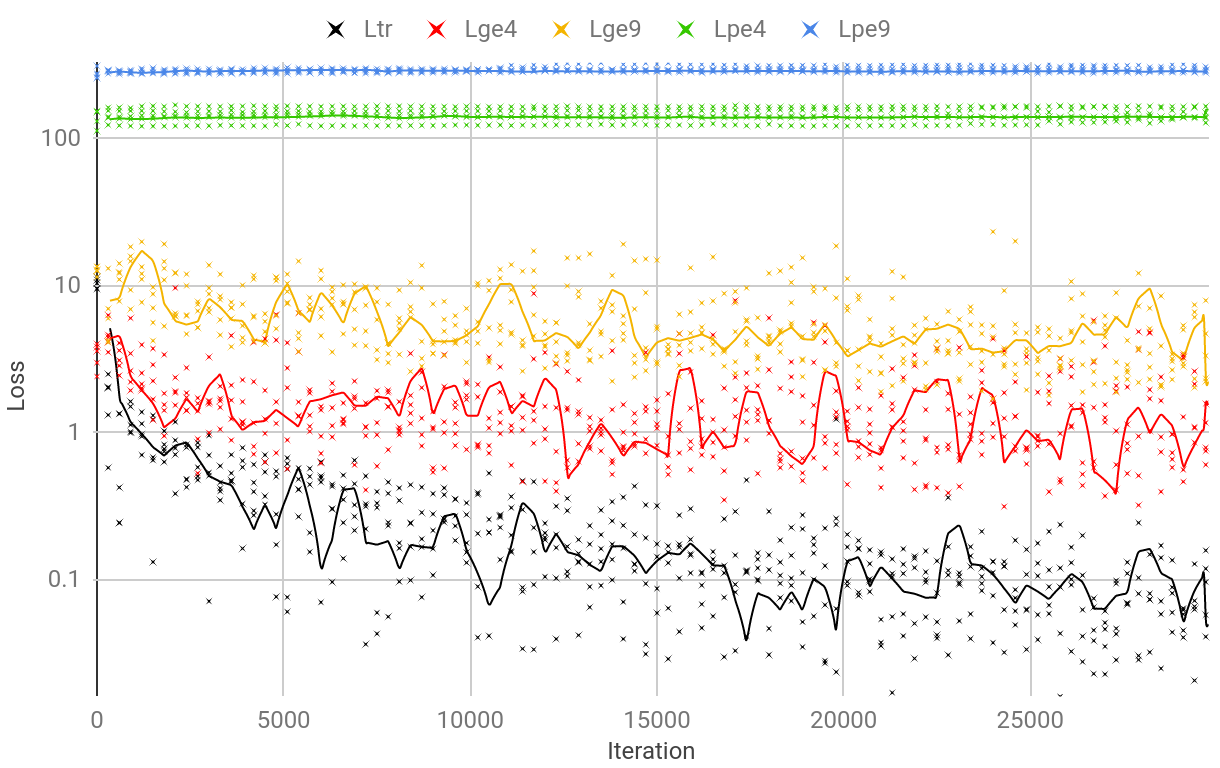
\includegraphics[width=.9\linewidth]{fig/content/results/physics/physics_base.png}
    \caption{Loss plot of the physics experiment with permutations only of the testing set}
    \label{fig:physics_base_results}
\end{figure}

\subsubsection {Permutation of the training and testing sets}

This experiment evaluated the algorithm’s performance on non-permuted and permuted testing data after training with permutations.

The results displayed in the loss plot (Fig.\ref{fig:physics_perm_results}) show smaller differences between non-permuted and permuted testing data. The reduction of loss for permuted graphs indicates that the algorithm actually learned to identify some permutations.

A possible explanation for this phenomenon is that the use of randomness for determining the position of masses in the system input increases the generalization capability of the network.

\begin{figure}[H]
    \centering
    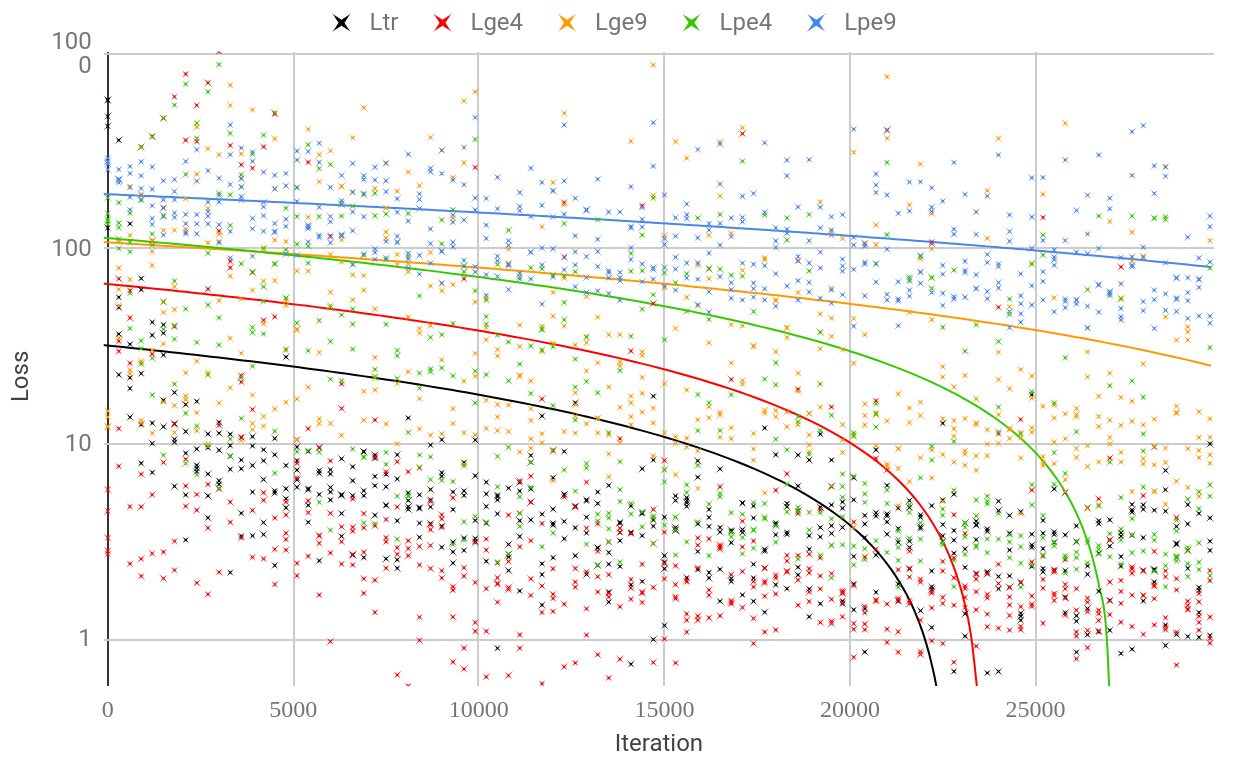
\includegraphics[width=.9\linewidth]{fig/content/results/physics/physics_perm.png}
    \caption{Loss plot of the physics experiment with permuted training and testing sets}
    \label{fig:physics_perm_results}
\end{figure}

\subsection{Experiments B - Shortest Paths}

\subsubsection {Permutation of the testing set}
    \begin{enumerate}[label=(\Alph*)]

        \item Infinite dataset
        \label{sec:infinite_test_only}
        
        An infinite dataset was used for the training and testing sets. At each iteration new graphs were randomly generated to train and test the network. The testing set was evaluated with and without permutations.
        
        The loss plot (Fig.\ref{fig:shotest_paths_base_results}) shows that the loss of the permuted testing set is the highest and, different from the loss of the non-permuted testing set, is not decreasing after iteration 75.
        
        And in the accuracy plot (Fig.\ref{fig:shotest_paths_base_ACC_results}) we can see that the network does not learn to identify the shortest path on the permuted testing set (the trend of the permuted testing set's accuracy is far from 1).
        
        \begin{figure}[H]
            \centering
            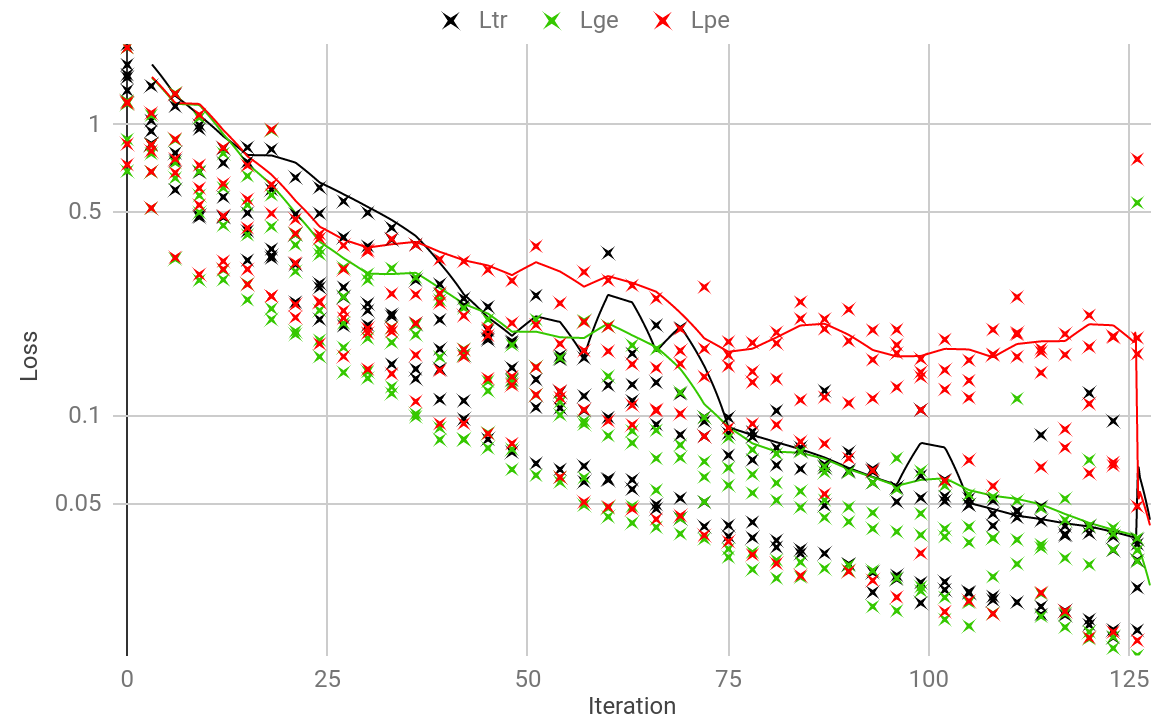
\includegraphics[width=.9\linewidth]{fig/content/results/shortest_path/base.png}
            \caption{Loss plot with infinite training set with permutations only of the testing set}
            \label{fig:shotest_paths_base_results}
        \end{figure}
        
        \begin{figure}[H]
            \centering
            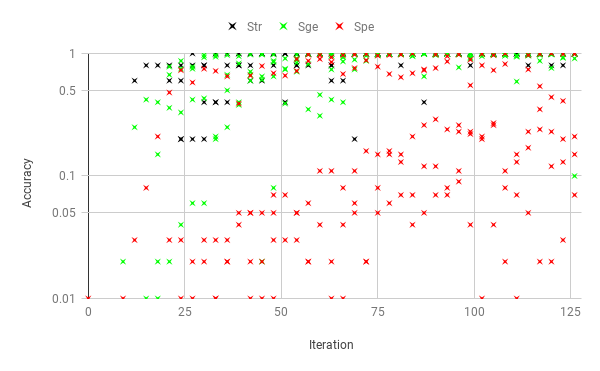
\includegraphics[width=.9\linewidth]{fig/content/results/shortest_path/base_ACC.png}
            \caption{Accuracy plot with infinite training set with permutations only of the testing set}
            \label{fig:shotest_paths_base_ACC_results}
        \end{figure}
        
        \item With epochs (every 25 iterations)
        \label{sec:epochs_test_only}
        
        To simulate a limited dataset, we reset the seed every 25 iterations, generating epochs. The testing set was evaluated with and without permutations.
        
        The loss plot (Fig.\ref{fig:shotest_paths_base_epochs_results}) shows that the loss of the permuted testing set is still the highest and, although it seems more uniform than Fig. \ref{fig:shotest_paths_base_results}, the trend shows that the results from configurations (A) and (B) are very similar.
        
        This similarity is also seen in the accuracy plot  (Fig.\ref{fig:shotest_paths_base_epochs_ACC_results}). The network did not learn to identify the shortest path on the permuted testing set (the trend of the permuted testing set's accuracy is far from 1).
        
        \begin{figure}[H]
            \centering
            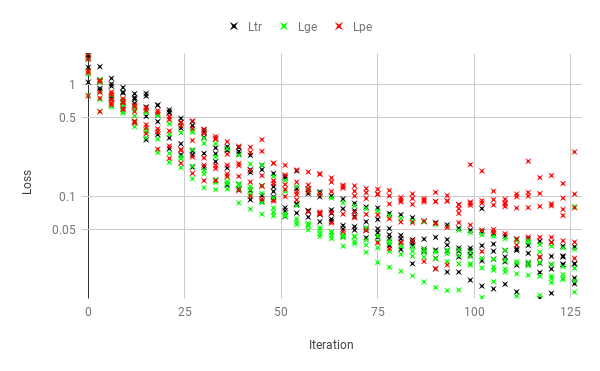
\includegraphics[width=.9\linewidth]{fig/content/results/shortest_path/epochs_base.png}
            \caption{Loss plot with training set repeating on every 25 iterations, with permutations only of the testing set}
            \label{fig:shotest_paths_base_epochs_results}
        \end{figure}
        
        \begin{figure}[H]
            \centering
            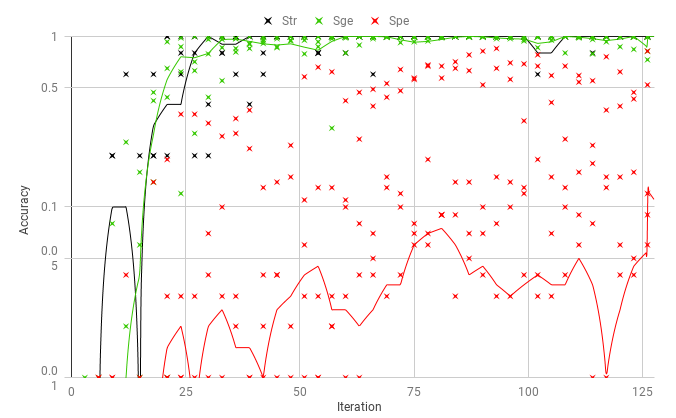
\includegraphics[width=.9\linewidth]{fig/content/results/shortest_path/epochs_base_ACC.png}
            \caption{Accuracy plot with training set repeating on every 25 iterations, with permutations only of the testing set}
            \label{fig:shotest_paths_base_epochs_ACC_results}
        \end{figure}

    \end{enumerate}

\subsubsection {Permutation of the training and testing sets}

\begin{enumerate}[label=(\Alph*)]

        \item Infinite dataset
        
        The difference from the subsection 5.2.1 \ref{sec:infinite_test_only} is that now we permuted the training set as well.
        
        The loss of the permuted testing set in Fig.\ref{fig:shotest_paths_train_perm_results} is lower than in Fig.\ref{fig:shotest_paths_base_results}. The permuted testing set's loss trend converges with the non-permuted testing set's loss trend.
        
        The accuracy plot (Fig.\ref{fig:shotest_paths_train_perm_ACC_results}) also shows an improvement in the networks' learning. We can see that now the network learns to identify the shortest path on the permuted testing set (the trend of the permuted testing set's accuracy reaches 1).
        
        \begin{figure}[H]
            \centering
            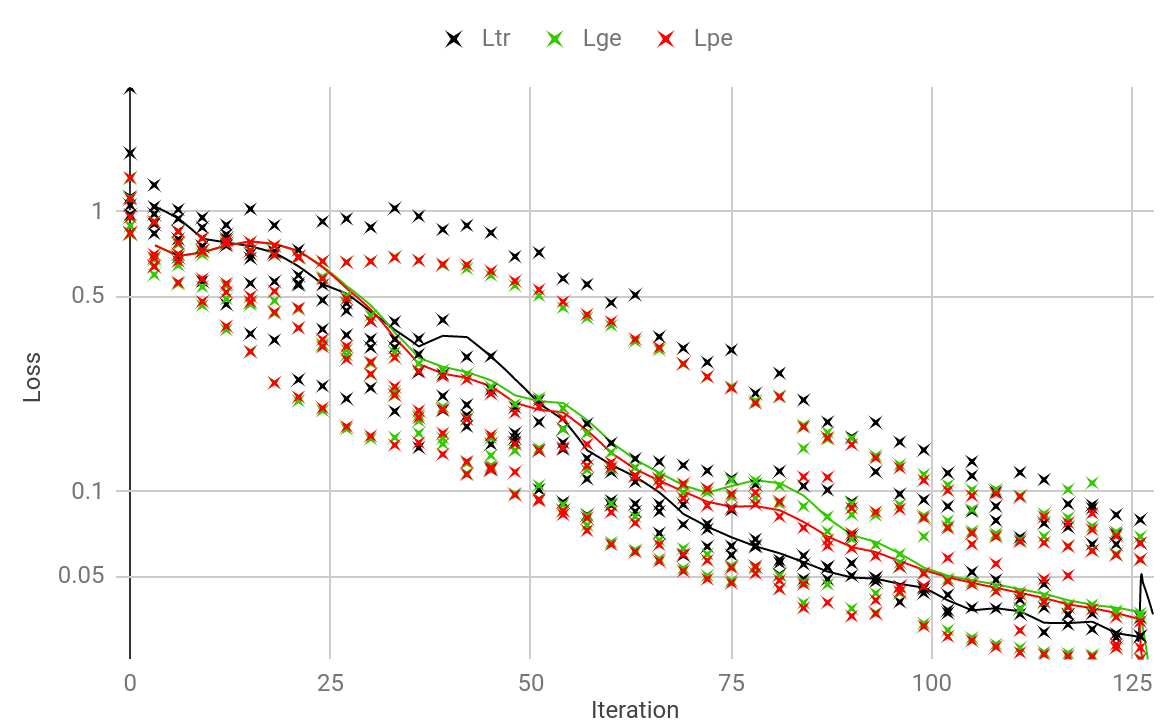
\includegraphics[width=.9\linewidth]{fig/content/results/shortest_path/training_perm.png}
            \caption{Loss plot with infinite permuted training set}
            \label{fig:shotest_paths_train_perm_results}
        \end{figure}
        
        \begin{figure}[H]
            \centering
            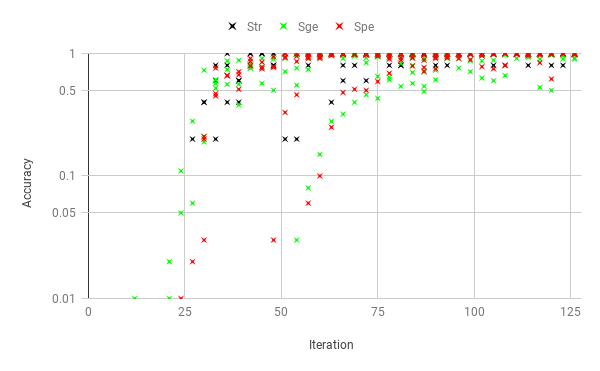
\includegraphics[width=.9\linewidth]{fig/content/results/shortest_path/training_perm_ACC.png}
            \caption{Accuracy plot with infinite permuted training set}
            \label{fig:shotest_paths_train_perm_ACC_results}
        \end{figure}
        
        \item With epochs (every 25 iterations)
        
        The difference from the subsection 5.2.1 \ref{sec:epochs_test_only} is that now we permuted the training set as well.
        
        The loss plot (Fig.\ref{fig:shotest_paths_epochs_perm_results}) shows that the trend of the loss of the permuted testing set also converges with the trend of the loss of the non-permuted testing set, similar to Fig. \ref{fig:shotest_paths_train_perm_results}.
        
        This similarity is also seen in the accuracy plot (Fig.\ref{fig:shotest_paths_epochs_perm_ACC_results}). The network learns to identify the shortest path on the permuted testing set (the trend of the permuted testing set's accuracy reaches 1).
        
        \begin{figure}[H]
            \centering
            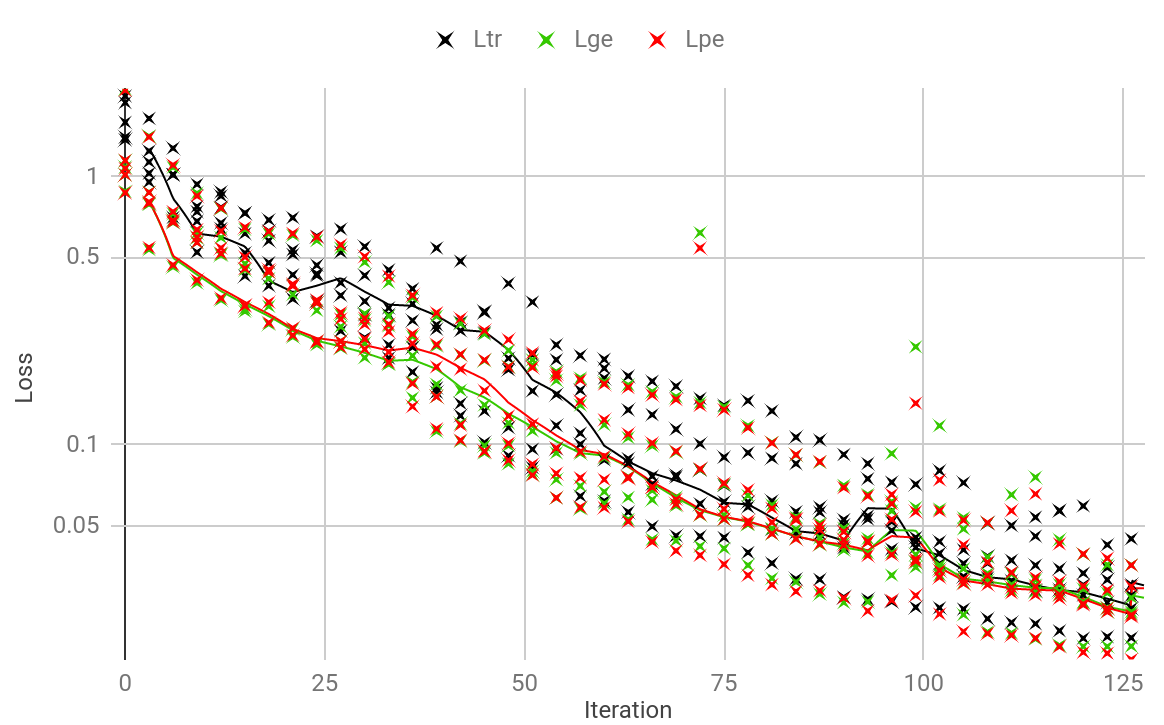
\includegraphics[width=.9\linewidth]{fig/content/results/shortest_path/epochs_perm.png}
            \caption{Loss plot with permuted training set repeating on every 25 iterations}
            \label{fig:shotest_paths_epochs_perm_results}
        \end{figure}
        
        \begin{figure}[H]
            \centering
            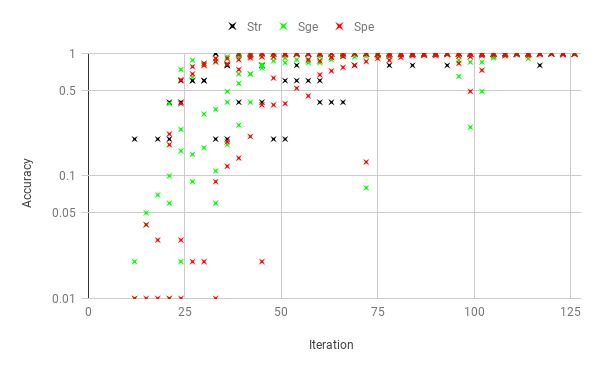
\includegraphics[width=.9\linewidth]{fig/content/results/shortest_path/epochs_perm_ACC.png}
            \caption{Accuracy plot with permuted training set repeating on every 25 iterations}
            \label{fig:shotest_paths_epochs_perm_ACC_results}
        \end{figure}
        
        \item Various permutations of the same training set (per epoch)
        
        To simulate a limited dataset, we reset the seed every 25 iterations, generating epochs. But now, on every iteration we generate a different permutation of the same dataset and train the network with it.
        
        Since we are training with different permutations of the same dataset, we expected the network to learn how to deal with permutations faster, but it does not seem to be the case (as we can see in the Loss plot from Fig.\ref{fig:shotest_paths_varios_perms_results}, which is very similar to the loss plot from Fig.\ref{fig:shotest_paths_epochs_perm_results}).
        
        However, in the accuracy plot (Fig.\ref{fig:shotest_paths_varios_perms_ACC_results}) the curves start to increase earlier compared to the accuracy plot from Fig.\ref{fig:shotest_paths_epochs_perm_ACC_results}. The network learns to identify the shortest path on the permuted testing set (the trend of the permuted testing set's accuracy reaches 1), as well.
        
        \begin{figure}[H]
            \centering
            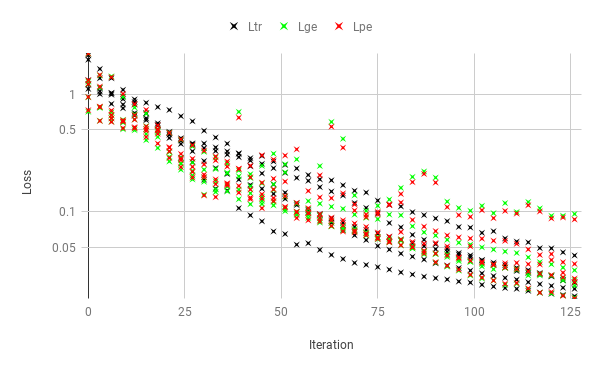
\includegraphics[width=.9\linewidth]{fig/content/results/shortest_path/various_perms_per_epoch.png}
            \caption{Loss plot training with various permutations per epoch}
            \label{fig:shotest_paths_varios_perms_results}
        \end{figure}
        
        \begin{figure}[H]
            \centering
            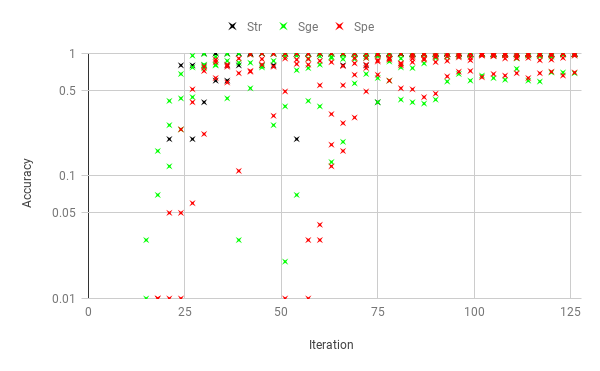
\includegraphics[width=.9\linewidth]{fig/content/results/shortest_path/various_perms_per_epoch_ACC.png}
            \caption{Accuracy plot training with various permutations per epoch}
            \label{fig:shotest_paths_varios_perms_ACC_results}
        \end{figure}

    \end{enumerate}
    
\subsection{Experiments C - Regions Separation}

\subsubsection {Permutation of the testing set}

\begin{figure}[H]
    \centering
    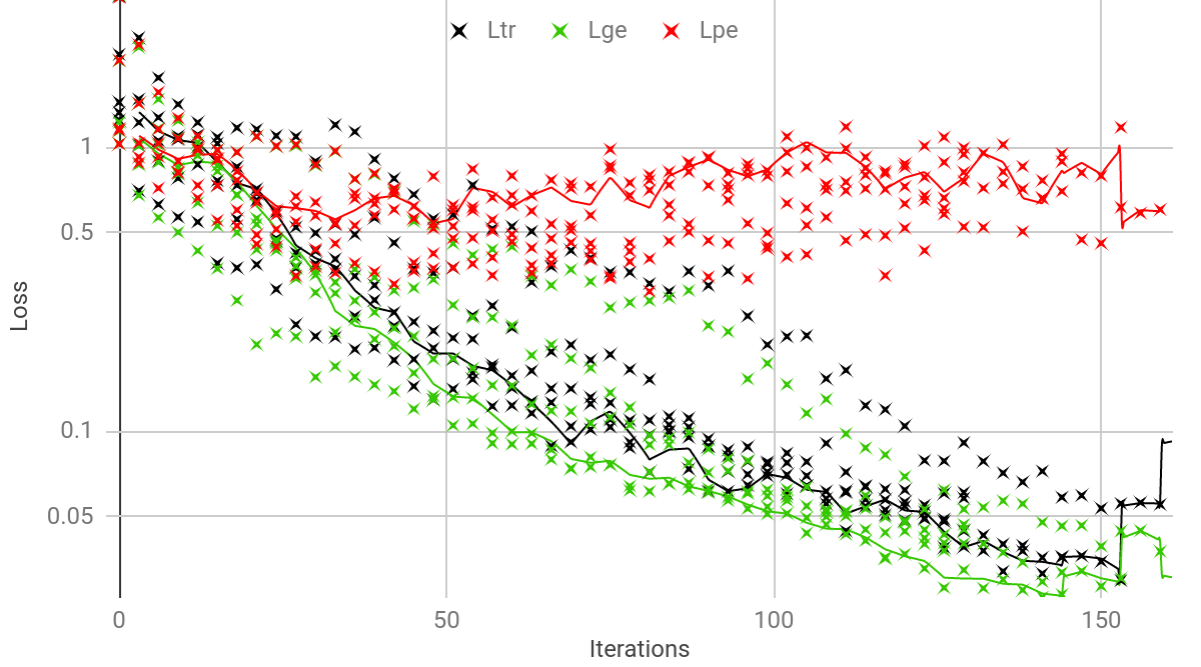
\includegraphics[width=.9\linewidth]
    {fig/content/results/shapes/base/loss.png}
    \caption{Loss plot of the experiments without permutations in the training set}
    \label{fig:regions_separation_base_loss}
\end{figure}

Without permutations in the data structure representation of the graphs in the training set (Fig. \ref{fig:regions_separation_base_loss}), we can observe a clear separation between the loss of permuted testing set and non-permuted testing set in the representation, which suggests, at least in this case, the algorithm is not invariant with respect to those permutations in the data structure representation of the graphs.

\begin{figure}[H]
    \centering
    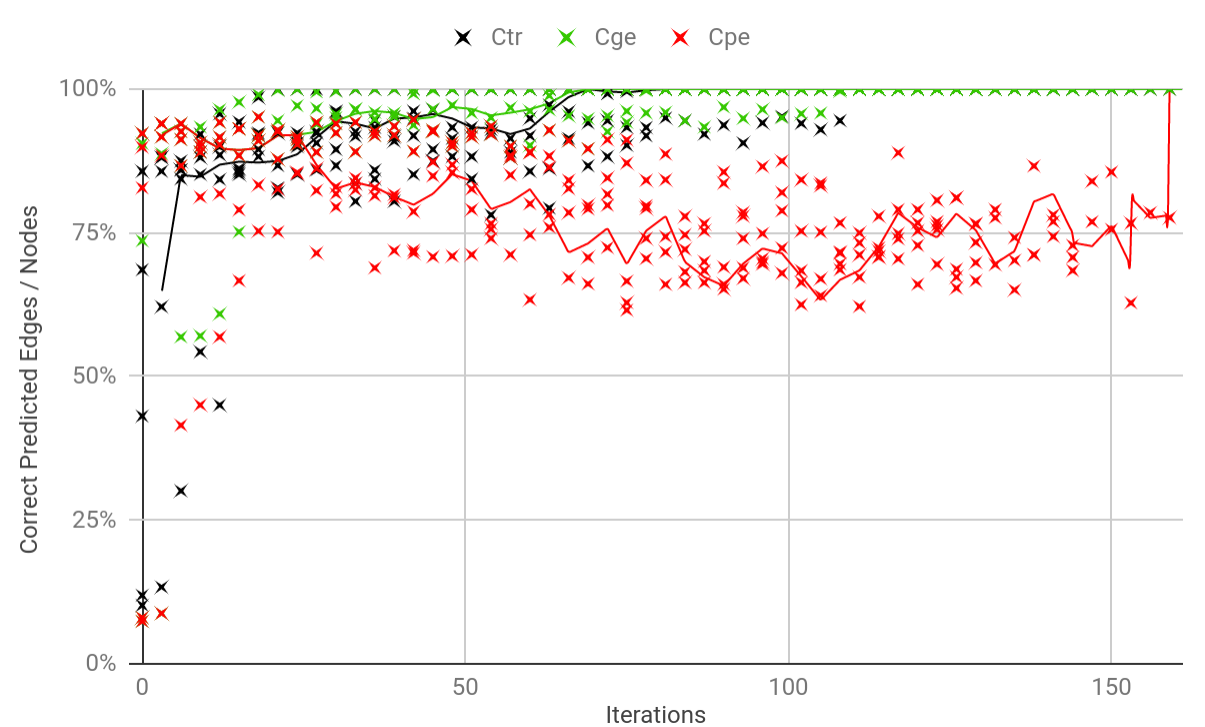
\includegraphics[width=.9\linewidth]
    {fig/content/results/shapes/base/correct.png}
    \caption{Accuracy plot of the experiments without permutations in the training set}
    \label{fig:regions_separation_base_accuracy}
\end{figure}

Analysing the accuracy plot considering the proportion of correct predicted nodes and edges (Fig.\ref{fig:regions_separation_base_accuracy}) in the case of non-permuted training set, we can see that non-permuted testing set's accuracy reached 100\% but the permuted testing set's accuracy didn't. In fact accuracy slightly decreases after the first peak.

\subsubsection {Permutation of the training and testing sets}

\begin{figure}[H]
    \centering
    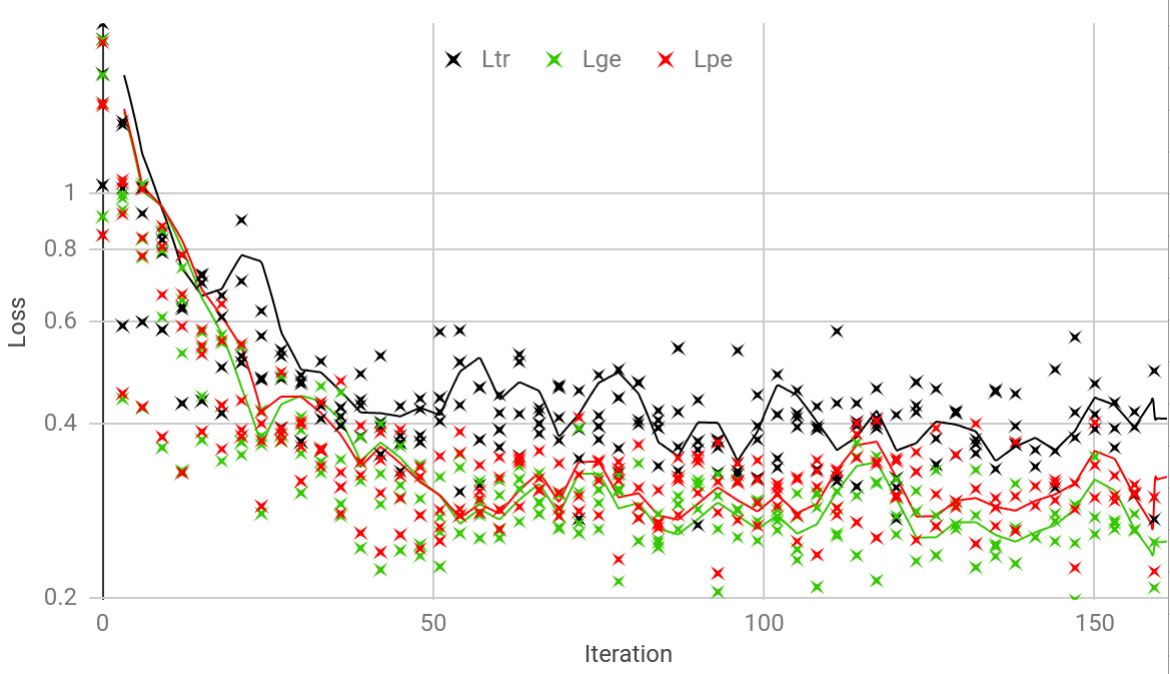
\includegraphics[width=.9\linewidth]
    {fig/content/results/shapes/permuted_training/loss.png}
    \caption{Loss plot of the experiment with permutations in the training set}
    \label{fig:regions_separation_permuting_training_loss}
\end{figure}

Permuting the representations of the training set (Fig. \ref{fig:regions_separation_permuting_training_loss}), even though the difference between Lge and Lpe is greatly reduced in comparison with the previous experiment (without permutations in training), we can see that no loss gets below 0.2 when in the previous one, they get below 0.05 which suggests a significant reduction in the performance of the network.

\begin{figure}[H]
    \centering
    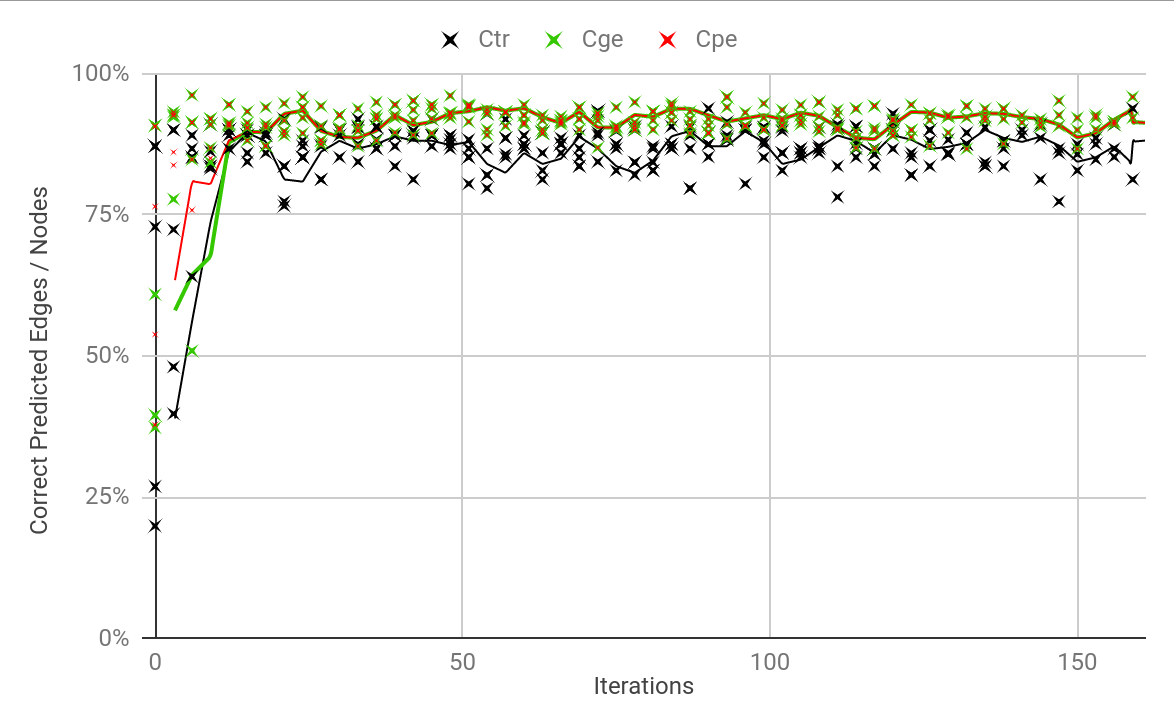
\includegraphics[width=.9\linewidth]
    {fig/content/results/shapes/permuted_training/correct.png}
    \caption{Accuracy plot of the experiment with permutations in the training set}
    \label{fig:regions_separation_permuting_training_accuracy}
\end{figure}

Analysing the accuracy plot (Fig. \ref{fig:regions_separation_permuting_training_accuracy}) in the case of permuted training set, we can see that nor Cpe neither Cge reach 100\%, which means that none of them actually learned to solve the problem completely in the time box available. 




\section{Conclusions}

In the experiments we carried out, it was possible to verify meaningful differences in learning between non-permuted and permuted testing sets, where permuted testing sets caused some networks to perform poorer.

Also, the difference in the losses of the the permuted and non-permuted testing sets with non-permuted training set seems to have a relationship with the pattern in the data structure representation of the graphs. 

In the Regions Separation experiment, this difference seems to be the greatest, because the non-permuted representation stores every pixel in an specific order.

In the Physics experiment, this difference can be explained by the fixed masses which in the non-permuted representation are always the first and the last masses.

In the Shortest Paths experiment, this difference is not so representative. This can be explained by the way in which the graphs are generated, randomly with a modified geographic threshold algorithm.

In all these experiments, we explored a possible improvement for the invariance problem in graph representation where the use of permuted training sets achieved better results.

{\small

\bibliographystyle{bib/IEEEtran}
\bibliography{bib/bib.bib}
}

%\section{Appendix}

%\subsection{Physics Experiments}

%\subsection{Shortest Paths Experiments}

%\subsection{Regions Separation Experiments}


\end{document}
